\section{Exploratory Data Analysis} \label{ch4:exploratory}

\subsection{Backlog of Issues per Addressed Issue}

\begin{figure}
	\centering
	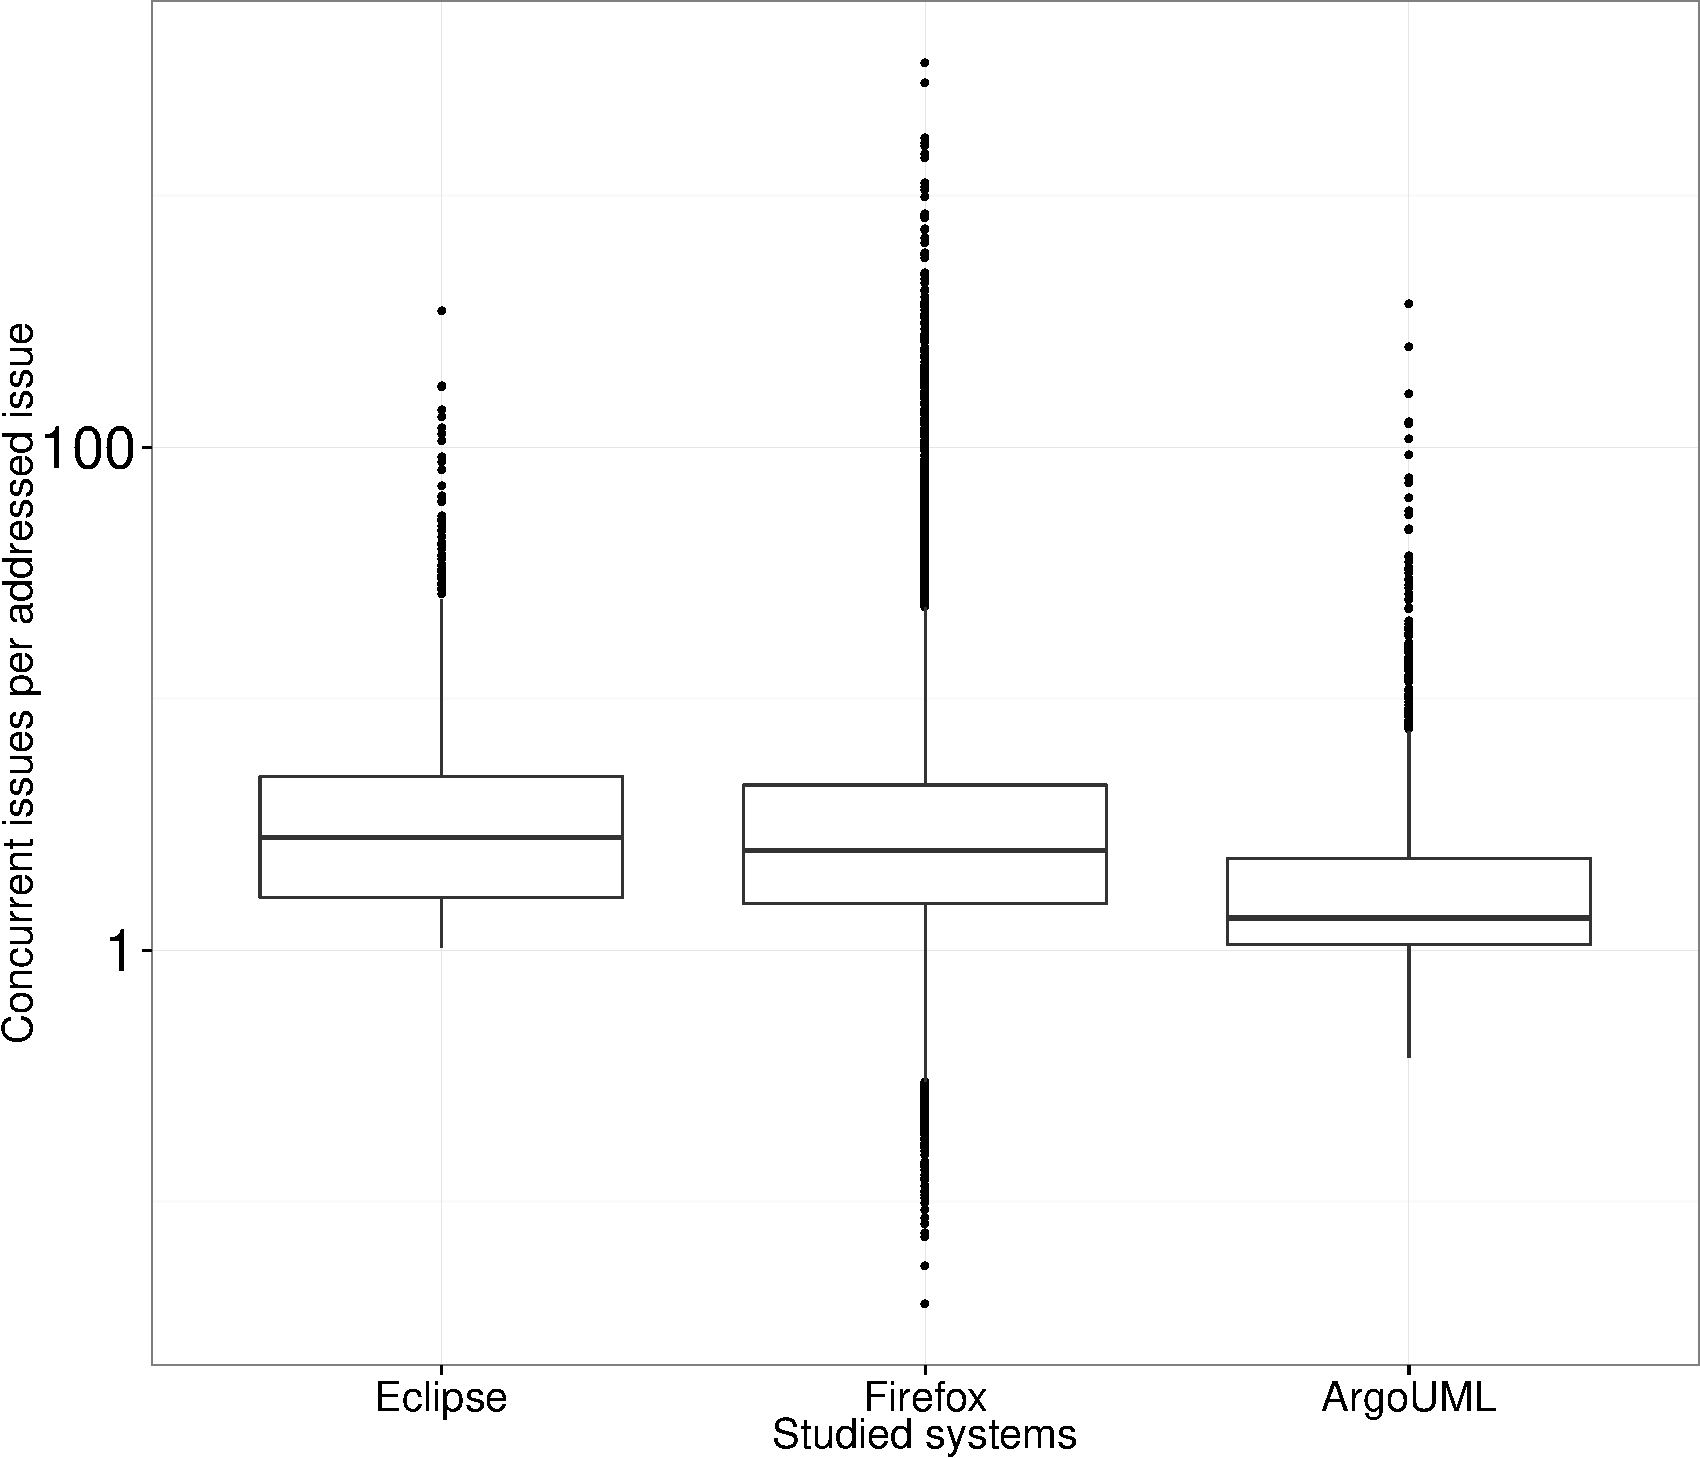
\includegraphics[width=0.85\textwidth,keepaspectratio]
	{chapters/chapter4/figures/boxplot-workloadratio-system.pdf}
	\caption{\textbf{Backlog of issues per addressed issue of the current
		release cycle.} The median number of concurrent fixes per addressed issue
	for the Eclipse, Firefox, and ArgoUML projects are 3, 2, and 1, respectively.}
	\label{ch4:fig:concurrent_issues}
\end{figure}

Since we observe that the integration workload in terms of the number of
backlog of issues is an influential attribute in all of the studied projects, we
also investigate the competition that is due to issues that are waiting for
integration per addressed issue in the release cycle.
\hyperref[ch4:fig:concurrent_issues]{Figure}~\ref{ch4:fig:concurrent_issues} shows the
distributions of the number of competing issues for an addressed issue of a
given release cycle. For each addressed issue, a median of three, two, and one
other issues are competing for integration in the Eclipse, Firefox, and ArgoUML
projects, respectively. It is interesting to note that the distribution of the
Firefox project is equivalent to the Eclipse project one, even though the
Firefox releases are more frequent. This might suggest an intense period of
activity in the Firefox release cycles (high rates of integration and fixing activity).

\subsection{Practical Suggestions}

In our study, we observe that attributes such as: \textit{fixing time per
resolver}, \textit{backlog of issues}, \textit{resolver integration speed}, and
\textit{queue position} have a considerable impact on the studied types of
delivery delay. As such, we suggest that our investigated attributes could be
used as a starting point in project management tools to track the \DIFdelbegin \DIFdel{integration
time }\DIFdelend \DIFaddbegin \DIFadd{delivery
delay }\DIFaddend of addressed issues. For example, a tool that could automatically track the
\textit{backlog of issues} by using the ITS, could raise warnings when the
backlog for integration crosses a project-specific threshold. Such a warning
could lead to early integration sessions before the official release deadline,
and prevent log jams in the integration queue. 

Our work suggests that the integration \DIFdelbegin \DIFdel{stage is }\DIFdelend \DIFaddbegin \DIFadd{and delivery stages are }\DIFaddend also a bottleneck
that has to be managed in a software project. Tracking data and developing tools
to reduce delivery delay should also be the target of the practice and research.

